% ============================================================
\section{Evaluation}
\label{sec:evaluation}

This chapter evaluates the system with a single goal: quantify pose consistency in a \emph{common camera frame} so that pose-estimation error can be separated from world-space alignment error caused by registration and tracking. The analysis is built on paired requests computed from the same scene instance using two pipelines: a RealSense reference pipeline and an AVP/UxPlay-view pipeline that uses RealSense depth reprojected into the mirrored AVP view.

\subsection{Evaluation Strategy}
\label{subsec:eval_strategy}

Two pipelines are compared that use the same pose estimator (FoundationPose) and the same object model, but differ in the camera view and depth input used for inference.

\begin{itemize}
    \item \textbf{RS--FoundationPose (reference).} Pose is estimated directly in the RealSense color camera frame using aligned RealSense RGB-D and a circular ROI mask defined in the RealSense view.
    \item \textbf{RS$\rightarrow$UxPlay--FoundationPose (evaluated).} Pose is estimated in the UxPlay (mirrored AVP) camera frame using UxPlay RGB and RealSense depth reprojected into the UxPlay view. The ROI is defined by normalized parameters in the UxPlay image plane. The resulting pose is then transformed back into the RealSense frame for comparison against the reference estimate.
\end{itemize}

Paired samples are collected so both pipelines process approximately the same scene instance. For reproducibility, request/response folders can be saved during capture and later replayed deterministically, which is useful for regression testing and for isolating failures that depend on specific inputs.

Figure~\ref{fig:rs_reference_pose} shows an example output from the reference pipeline, visualized by projecting the estimated pose back into the RealSense color view.

\begin{figure}[H]
\centering
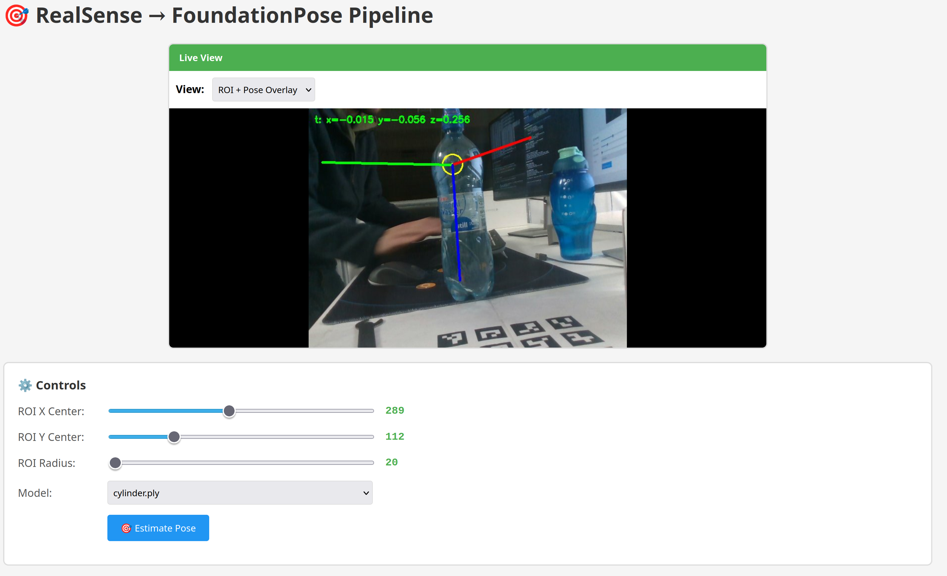
\includegraphics[width=\textwidth]{figures/RS_FP_pipeline.png}
\caption[RS reference pose]{Object pose output from the RealSense reference FoundationPose request.}
\label{fig:rs_reference_pose}
\end{figure}

\subsection{Pose Error Metrics}
\label{subsec:eval_metrics}

Each paired sample yields two poses that are compared in the \emph{RealSense} frame: the reference pose $\mathbf{T}^{\text{ref}}_{RS \leftarrow O}$ and the evaluated pose $\mathbf{T}^{\text{eval}}_{RS \leftarrow O}$ (obtained by transforming the UxPlay-frame result back to $RS$). Let $\mathbf{t}_{\text{ref}}, \mathbf{t}_{\text{eval}}$ be the translation vectors and $\mathbf{R}_{\text{ref}}, \mathbf{R}_{\text{eval}}$ the rotation matrices. Translation error is computed as
\[
e_t = \|\mathbf{t}_{\text{ref}} - \mathbf{t}_{\text{eval}}\|_2,
\]
and rotation error is computed from the relative rotation
\[
\Delta \mathbf{R} = \mathbf{R}_{\text{ref}} \mathbf{R}_{\text{eval}}^\top,
\qquad
e_r = \cos^{-1}\left(\frac{\mathrm{trace}(\Delta \mathbf{R})-1}{2}\right).
\]
These metrics quantify disagreement in the estimated object pose while remaining independent of any world-space anchoring. They therefore isolate the effect of reprojection and camera-view differences on pose inference.

\subsection{Interpreting World-Space Overlays}
\label{subsec:eval_worldspace}

Camera-frame agreement is necessary but not sufficient for visually accurate overlays in immersive space. Once a pose is rendered in AVP world coordinates, additional error sources enter the pipeline that are deliberately excluded from the camera-frame metrics. In particular, noise in ArUco detection and extrinsic estimation perturbs the camera-to-camera transform $\mathbf{T}_{AVP \leftarrow RS}$, affecting both depth reprojection and the subsequent coordinate lifting used for visualization. Any mismatch in the UxPlay camera model (intrinsics and distortion) introduces systematic projection bias that can manifest as a consistent offset even when the underlying pose estimate is stable. On top of this, ARKit device/head tracking can drift over time, shifting the world anchor relative to the physical scene. Finally, small errors in the calibrated device-to-camera offset can dominate perceived misalignment because they directly affect the mapping from camera-frame outputs into world space.

Consequently, a pose may remain stable and self-consistent in the image plane while still appearing shifted or drifting in immersive space. World-space overlays should therefore be interpreted as an end-to-end sanity check of the full registration and tracking stack rather than a direct measure of pose inference quality.


\subsection{Transformed Depth Quality}
\label{subsec:eval_depth_quality}

The evaluated pipeline introduces an additional uncertainty source: reprojection of RealSense depth into the UxPlay view. Figure~\ref{fig:depth_transform_error} compares the aligned RealSense depth image and the depth map after transformation into the UxPlay camera frame. This example was captured with a relatively constrained baseline to keep the shared marker visible in both views.

In practice, small errors in camera-to-camera registration or imperfect intrinsics/distortion can produce local warping, sparse holes, and depth discontinuities after reprojection. If the ROI intersects these regions, FoundationPose receives incomplete or inconsistent depth, which can reduce stability or increase jitter.

\begin{figure}[H]
\centering
\includegraphics[width=\textwidth]{figures/rs_depth_vs_transformed_depth.png}
\caption[Depth reprojection comparison]{Aligned RealSense depth (left) and depth reprojected into the UxPlay view (right) for the same scene instance.}
\label{fig:depth_transform_error}
\end{figure}

\subsection{Registration and Overlay Sanity Checks}
\label{subsec:eval_overlay_checks}

Registration is validated through overlay inspection at two levels.

\paragraph{Image-plane validation (UxPlay view).}
The UxPlay view is used to confirm that estimated transforms yield coherent overlays in the mirrored image plane. Figure~\ref{fig:rs_pose_overlay_uxplay} shows the RealSense camera pose visualized as an overlay in the UxPlay view. This acts as a direct sanity check that the estimated registration outputs are consistent with the mirrored RGB content.

\begin{figure}[H]
\centering
\includegraphics[width=\textwidth]{figures/uxplay_rs_pose_overlay.png}
\caption[RealSense pose overlay in UxPlay]{UxPlay view with the estimated RealSense camera pose visualized as an overlay for registration validation.}
\label{fig:rs_pose_overlay_uxplay}
\end{figure}

\paragraph{Marker and object overlays (UxPlay and immersive).}
The same mechanism is used to visualize ArUco-related overlays and object pose overlays in the image plane. Figure~\ref{fig:aruco_overlay_uxplay} illustrates combined ArUco and RealSense overlays, while Figure~\ref{fig:object_pose_uxplay} shows an object pose overlay rendered on the mirrored feed. Figure~\ref{fig:pose_overlay_3d} shows the corresponding immersive 3D overlays; any remaining misalignment should be interpreted as a combination of registration error and tracking drift rather than pose inference alone.

\begin{figure}[H]
\centering
\includegraphics[width=0.95\textwidth]{figures/.png}
\caption[ArUco and RS overlays]{ArUco and RealSense overlays rendered in the UxPlay view.}
\label{fig:aruco_overlay_uxplay}
\end{figure}

\begin{figure}[H]
\centering
\includegraphics[width=0.95\textwidth]{figures/object_pose_overlay_uxplay.png}
\caption[Object pose overlay in UxPlay]{Object pose overlay rendered in the UxPlay view for camera-frame verification.}
\label{fig:object_pose_uxplay}
\end{figure}

\begin{figure}[H]
\centering
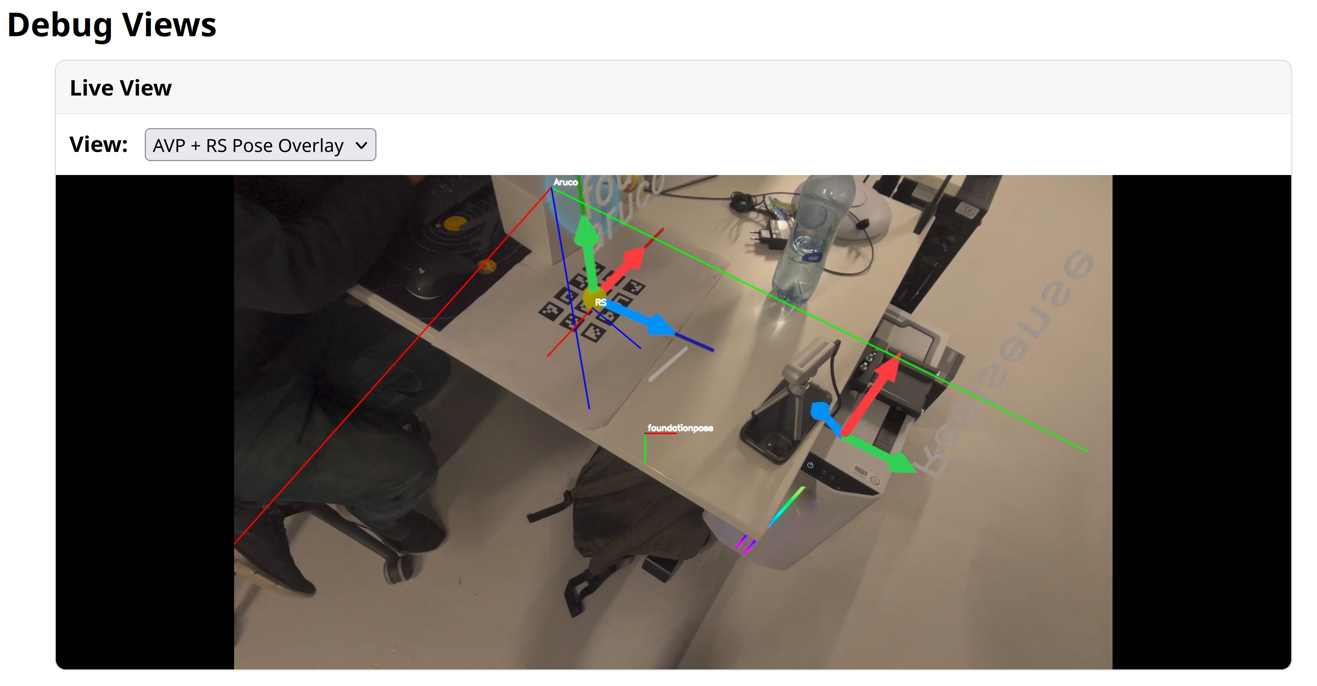
\includegraphics[width=0.9\textwidth]{figures/3d_pose_overlays_aruco_rs.png}
\caption[Immersive 3D overlays]{World-space pose overlays rendered in immersive space after registration and device-anchor lifting.}
\label{fig:pose_overlay_3d}
\end{figure}
\subsection{Observed Failure Modes}
\label{subsec:eval_failures}

Testing revealed a small set of recurring failure modes that consistently affected either the transformed RGB-D inputs, the stability of world-space overlays, or both. Table~\ref{tab:failure_modes} summarizes the dominant error sources and practical mitigation directions that follow directly from the current system architecture.
\begin{table}[H]
\centering
\caption{Observed failure modes and mitigation/outlook considerations (summarized, passive voice).}
\label{tab:failure_modes}
\begin{tabular}{p{0.30\linewidth}p{0.62\linewidth}}
\toprule
\textbf{Error source} & \textbf{Proposed mitigation / outlook} \\
\midrule
Depth reprojection artifacts (holes, local warping) &
More stable estimates of $\mathbf{T}_{AVP \leftarrow RS}$ are expected to be obtained through improved ArUco conditions (marker placement/size and quality gating) and refined UxPlay intrinsics/distortion calibration. Sparse depth is intended to be handled via ROI-aware validity masks and optional hole filling so that invalid regions are ignored during inference. \\
\midrule
Tracking drift in immersive mode (device/head anchor drift) &
World-space overlays are intended to be treated primarily as end-to-end feedback, while camera-frame metrics are prioritized for inference evaluation. Drift sensitivity is expected to be reduced by more frequent anchoring to a physical reference (periodic ArUco refresh) and by UI cues indicating anchor quality to trigger re-calibration when required. \\
\midrule
Calibration sensitivity (device-to-camera offset tuning) &
Manual offset tuning is intended to be replaced by a guided calibration procedure with quantitative alignment feedback and automatic refinement based on marker reprojection error. Calibrations are expected to be persisted per setup and safeguarded by consistency checks to detect invalid configurations. \\
\midrule
Recursive mirroring artifacts (infinite mirror from ROI/debug windows) &
Capture is intended to be performed without mirrored diagnostic/ROI windows visible, e.g., by using a snapshot-style ROI workflow and relocating debug views to non-mirrored displays. Backend-side detection of recursive frames is expected to be used to suppress ArUco updates when contamination is detected. \\
\bottomrule
\end{tabular}
\end{table}
